% -------------------------------------------------------------------------------------------------
% QUALITATIVE EVALUATION
% -------------------------------------------------------------------------------------------------
\section{Qualitative Evaluation}
\label{sec:qualitative_evaluation}
In this section, we will perform a qualitative evaluation of our solution with the other solutions,
such as full Virtual Machines and tools that implement the TOSCA standard. In our evaluation we
will compare the software required to provisioning the smart place infrastructure and also discuss
about the advantages of our solution compared with the others.

\subsection{Container-based vs. VM-based solution}
\label{sub:container_vs_vm_solution}
The provisioning of the RFID software in Cloud4Things is performed through Docker containers. The
decision to adopt this approach regards with the fact that we want our provisioned stack is as
small as possible, without the performance of our solution being affected. A alternative to
provisioning the RFID software stack is to use Virtual Machines. However, full VM presents
an overhead regarding the amount of resources that are consumed.

% Container vs. VM stack
\begin{figure}[!ht]
  \centering
  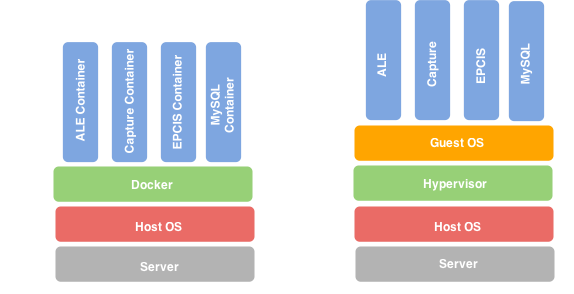
\includegraphics[width=.8\textwidth]{images/container-vs-vm-stack}
  \captionof{figure}{Container vs. VM stack}
\end{figure}

\textit{We need to compare the stack, and it will be good provides some metrics such as size of the
both stacks.}\\

\subsection{Cloud4Things vs. TOSCA-based tools}
\label{sub:c4t_vs_tosca}

In order to provisioning the smart place infrastructure with TOSCA, we need to have a special
provisioning engine for TOSCA. Currently there are several tools that implements
a provisioning engine for TOSCA such as Ubuntu Juju, Cloudify and the open-source
implementation OpenTOSCA.

We need to compare the advantages of our solution compared with TOSCA-based tools and also
what disadvantages our solution has compared with these tools.

\subsection{Preliminary Results}
\label{sub:preliminary_results}
